\documentclass[10pt,A4paper]{article}

\usepackage{acronym}
\usepackage{amsmath,amssymb}
\usepackage[aboveskip=1pt,labelfont=bf,labelsep=period,justification=raggedright,singlelinecheck=off]{caption}
\usepackage{changepage}
\usepackage{cite}
\usepackage{nameref,hyperref}
\usepackage[right]{lineno}
\usepackage[nopatch=eqnum]{microtype}

\usepackage{xcolor}

\usepackage[outputdir=out]{minted}
\definecolor{bg}{HTML}{282828} % fro https://github.com/kevinsawicki/monokai
\setminted{autogobble=true,bgcolor=bg,linenos=true,style=monokai}

\bibliographystyle{abbrv}

% Header and Footer with logo
\usepackage{lastpage,fancyhdr,graphicx}
\usepackage{epstopdf}
\pagestyle{fancy}
\fancyhf{}
\rfoot{\thepage/\pageref{LastPage}}
\renewcommand{\headrulewidth}{0pt}
\renewcommand{\footrule}{\hrule height 2pt \vspace{2mm}}
\lfoot{\today}

\newcommand{\etal}{{\textit{et al.}}}
\providecommand{\keywords}[1]{\textbf{Keywords } #1}


% Create acronyms to use in text
\newacro{ode}[ODE]{Ordinary Differential Equation}
\newacro{oed}[OED]{optimal experimental design}


\begin{document}
% ########################################################################
% ########################################################################
\vspace*{0.2in}
% Title must be 250 characters or less.
\begin{flushleft}
{\Large
\textbf\newline{Model Calibration with Process Variables depending on Environmental Parameters}}
\newline
\\
Polina Gaindrik\textsuperscript{1,2,3},
Jonas Pleyer\textsuperscript{1,2},
Christian Fleck\textsuperscript{1,2,3}
\\
\bigskip
\textbf{1} \href{https://www.fdm.uni-freiburg.de/spatsysbio}{University of Freiburg}\\
\textbf{2} \href{https://www.fdm.uni-freiburg.de/spatsysbio}{Freiburg Center for Data Analysis and Modeling}\\
\textbf{3} \href{https://tsenso.com/en/}{Tsenso}\\
\bigskip

\end{flushleft}
% ########################################################################
% ########################################################################
\section*{Abstract}
\linenumbers
Parameter estimation is a significant part of the model building that is always accompanied by quantification uncertainty.
Experimental design allows optimization of the observation conditions, reduces the uncertainty of the parameter estimation, and descreases the number of measurements. 
In this chapter, we provide instructions for finding the optimal experimental design using the (Baranyi and Roberts ?) growth model as an example. 
The guidelines are supposed to clarify the procedure and make it more accessible for a general reader of Systems Biology.
As an example, we provide a Python-written software that can be used for simple systems (??).

\keywords{Optimal experimental design, Parameter estimation, Fisher Information matrix, Identifiability, Uncertainty}

%
%
%
% ########################################################################
% ########################################################################
\section*{Introduction}
% \begin{figure}[h]
% 	\inputminted[linenos,firstline=57,lastline=79]{python}{../model-design-fischer-information-matrix/pool_model.py}
% 	\caption{Sample code written in Python~\cite{rossumPythonLanguageReference2010}.}
% \end{figure}
%
\begin{enumerate}
	\item Why do we want parameter estimation and experimental design?
	\item Flow-Chart Experimental Design
	\item Citations to common methods
\end{enumerate}


Mathematical modeling is a widely used tool to describe, understand and predict further behavior of living systems.
In particular, in the field of Predictive Biology, one can find a large variety of works that dwell on building models of different levels of complexity controlled by model parameters, e.g., to describe bacteria growthBased on a chosen model structure, these parameters can be estimated from the gathered experimental data.
Taking into account that the real experimental data always contains measurement noise, the parameter estimates can be only provided with some uncertainty. 
To decrease the error of the parameter values, not only enough experimental data should be gathered but the quality of this data is also pretty sufficient.
That rises quite an important question of finding the \ac{oed} where optimized experimental conditions and/or times allow one to reduce the number of measurements without loss of information thus sparing an effort of experimenters \cite{derlindenImpactExperimentDesign2013, balsa-cantoe.bangaj.r.COMPUTINGOPTIMALDYNAMIC2008}. 
In general, \ac{oed} can be used not only for the parameter estimation of the model but also for model discrimination to choose between different model structures \cite{kreutzSystemsBiology2009, stamatiOptimalExperimentalDesign2016}.
However, in this chapter, we would like to cover more deeply the methods for improving the parameter estimation of the model.
According to this, using tools of Statistics and specifically the Fisher information, several criteria were developed to assess data quality. 
The review of these different possible criteria the reader can find for example in works \cite{atkinsonDevelopmentsDesignExperiments1982, franceschiniModelbasedDesignExperiments2008}.
Depending on the goal, a researcher faces an important choice which among these sometimes contradicting each other criteria is the most suitable one for a particular case.
On the other hand, using the multi-objective approach, some attempts were made to improve the experimental design by combining these criteria \cite{telenOptimalExperimentDesign2012, logistRobustMultiobjectiveOptimal2011}.
If we are talking about predictive microbiology, one of the promising applications of the \ac{oed} is to optimize the temperature profile with the time of the experiment as it was done by García \etal \cite{garciaQualityShelflifePrediction2015} and Versyck \etal \cite{versyckIntroducingOptimal1999}.
Or, for example, Balsa-Canto \etal compared equidistant and optimized measurement times for such bacteria growth models as Baranyi and Roberts model and Bigelow model and have shown improvement in the latter case \cite{balsa-cantoe.bangaj.r.COMPUTINGOPTIMALDYNAMIC2008}.

\begin{figure}[H]
    \centering
    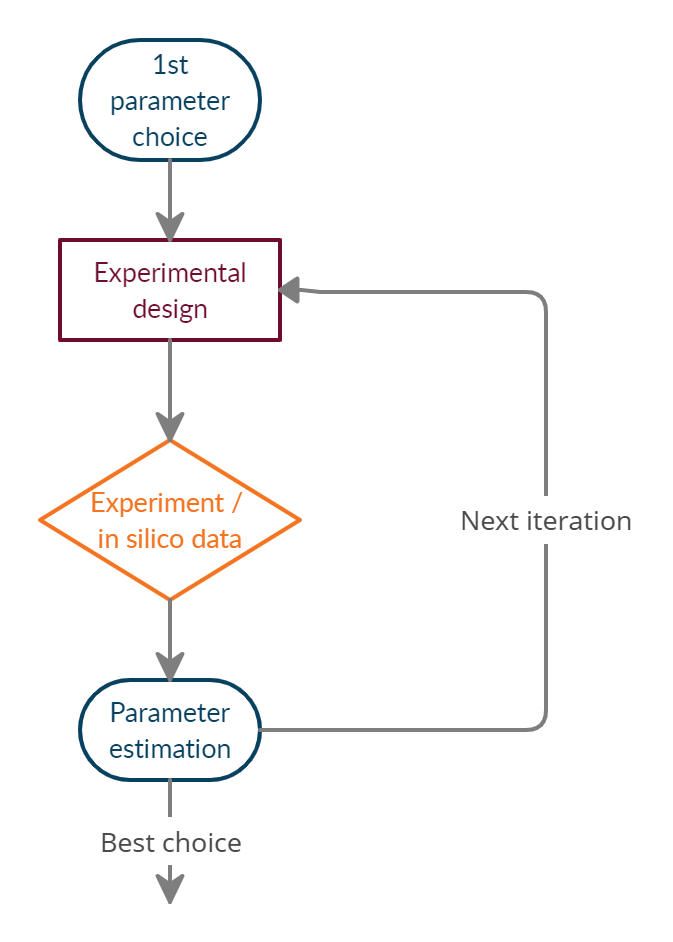
\includegraphics[scale=0.3]{Figures/scheme.png}
    \caption{The iterative process of model optimization for parameter estimation.}
    \label{fig:expdesign_scheme}
\end{figure}
In the beginning, we would like to briefly describe the whole iterative process of model building (see Fig. \ref{fig:expdesign_scheme}).
First of all, based on the literature review or some prior data from pilot experiments the first parameter estimation of the chosen model structure should be done.
The obtained values can be applied to propose the first optimal experimental design accounting for different constraints, e.g., the lab limitations, human resources, etc. 
Depending on availability, either real or numerical experiment should be conducted based on this design to gather measurement or in-silico data. 
This new data can be used for the new parameter estimations values with corresponding uncertainties.
After this, using new parameter values, the process can be repeated several times to increase the precision of the parameter estimates till the desired accuracy is achieved.







%
%
%
% ########################################################################
% ########################################################################
\section*{Materials and Methods}
This tutorial expects a working installation of the popular scripting language Python $\geq3.7$~\cite{rossumPythonLanguageReference2010}.
For installation instructions, please refer to the website \href{https://www.python.org/downloads/}{python.org}.
We have developed \mintinline[bgcolor=white,style=emacs]{bash}{FisInMa}, which is a set of tools to calculate the Sensitivity and Fischer Information Matrix and do parameter space exploration in order to find optimal results.
Users can obtain it by installing \mintinline[bgcolor=white,style=emacs]{bash}{FisInMa} from \href{https://pypi.org/project/FisInMa/0.0.1/}{pypi.org}.
The python website has guides for installing packages \href{https://packaging.python.org/en/latest/tutorials/installing-packages/}{packaging.python.org/}.
Most Unix-Based systems (eg. GNU/Linux) and Mac-OS can use \mintinline[bgcolor=white,style=emacs]{bash}{pip}
\begin{minted}[bgcolor=white]{bash}
pip install FisInMa
\end{minted}
or \mintinline[bgcolor=white,style=emacs]{bash}{conda} to install the desired package.
\begin{minted}[bgcolor=white]{bash}
conda install FisInMa
\end{minted}
%
%
% ########################################################################
\subsection*{Model Formulation}
\subsubsection*{Theory}
\begin{enumerate}
    \item Define ODE, Jacobian
    \item Which parameters are present?
    \item Differnce between Q-Values, P-Values, Const
\end{enumerate}
\subsubsection*{Code}
\begin{enumerate}
    \item Write ODE, Jacobian functions in python with Q, P, Const\\
    \mintinline[bgcolor=white,style=emacs]{python}{def ode_func(y, t, Q, P, Const):}\\
    \mintinline[bgcolor=white,style=emacs]{python}{def jacobian(y, t, Q, P, Const):}
    \item Define initial values \mintinline[bgcolor=white,style=emacs]{python}{(y0, t0)}
\end{enumerate}
%
% ########################################################################
\subsection*{Parameter Estimation}
\subsubsection*{Theory}
\begin{enumerate}
    \item Log-Likelihood Function
    \item Maximum-Likelihood Estimators
    \item Likelihood Function for Gaussian Noise
\end{enumerate}
\subsubsection*{Code}
\begin{enumerate}
    \item \mintinline[bgcolor=white,style=emacs]{python}{def likelihood_function(fitted_parameter, measurement_data)}
    \item \mintinline[bgcolor=white,style=emacs]{python}{scipy.optimize.minimize}
\end{enumerate}
%
% ########################################################################
\subsection*{Experimental Design}
\subsubsection*{Theory}
\begin{enumerate}
    \item Fischer, Sensitivity Matrix
    \item Observables: Determinant, Eigenvalues, etc.
\end{enumerate}
\subsubsection*{Code}
\begin{enumerate}
    \item How does the user calculate the Fischer Observable?
    \begin{minted}{python}
        def calculate_Fischer_observable(
            parameter_combinations,
            sensitivity_ode_function,
            y0_t0,
            jacobi,
            observable):
    \end{minted}
    \item How do we optimize for best results?
    \begin{minted}{python}
        def optimize_parameters(
            parameter_combinations,
            observable):
    \end{minted}
\end{enumerate}
%
%
%
% ########################################################################
% ########################################################################
\section*{Conclusion}
\begin{enumerate}
    \item Plots: Optimized time points
    \item Observable vs number of measurements
    \item Performance (scaling, limitations, etc.)
    \item 
\end{enumerate}
%
%
%
% ########################################################################
% ########################################################################
\section*{Supporting information}
%
%
%
\nolinenumbers
% ########################################################################
% ########################################################################
\bibliography{predictive-microbiology-software}

\end{document}
